\chapter{Resultados}

\section{Resultados durante la fase exploratoria}

Inicialmente, una vez probado el videojuego hasta terminar el nivel o llevar 12 minutos jugando, se le preguntaba al usuario con conocimiento experto cuánta usabilidad le daban al juego en una escala del 1 al 10.

Se hicieron tres iteraciones con esta metodología, además de aceptar los comentarios abiertos. En la primera fase, el promedio de usabilidad con 4 usuarios fue 2.5.

Posteriormente, una vez añadidas las implementaciones sugeridas anteriormente, la usabilidad ascendió a 6 con un tamaño muestral de 4, pero los usuarios reportaban que era muy fácil cometer errores, además de que la monotonía del juego y el tener que leer mucho producían mucha insatisfacción, pese a que era comprensible qué se podía hacer.

Finalmente, antes de probar con el público objetivo, se hizo una última prueba de usuario con un tamaño muestral de 6, obteniendo en promedio un puntaje de 8 sobre 10. En este caso los usuarios reportaron problemas menores, principalmente asociados a la interpretabilidad de ciertas animaciones o a la falta de estímulos, como la indicación de apretar ENTER para avanzar en el código.

\section{Resultados de la fase de evaluación académica}

\subsection{Prueba académica}

Las 15 personas que hicieron la prueba tuvieron ambas respuestas correctas, identificando correctamente el recorrido BFS y DFS en cada caso.

\subsection{Formulario MEEGA+: Percepción de usuario}

% Hablar de la suma de puntaje y puntaje promedio para los dos casos: De fase exploratoria y fase posterior.
% Poner acá gráficos y demás
Según \cite{meegaplus} un set de respuestas de un individuo se considera correcto y válido cuando tiene más del 85\% de las preguntas contestadas. En este caso no hubo omisiones.

En la figura \ref{RespuestasAgregadas} se muestran los resultados agregados para cada pregunta en cada categoría. Las preguntas se acortaron con acrónimos, pero la indexación está disponible en el anexo A \ref{AnexoA}.

\begin{figure}[h]
	\centering
	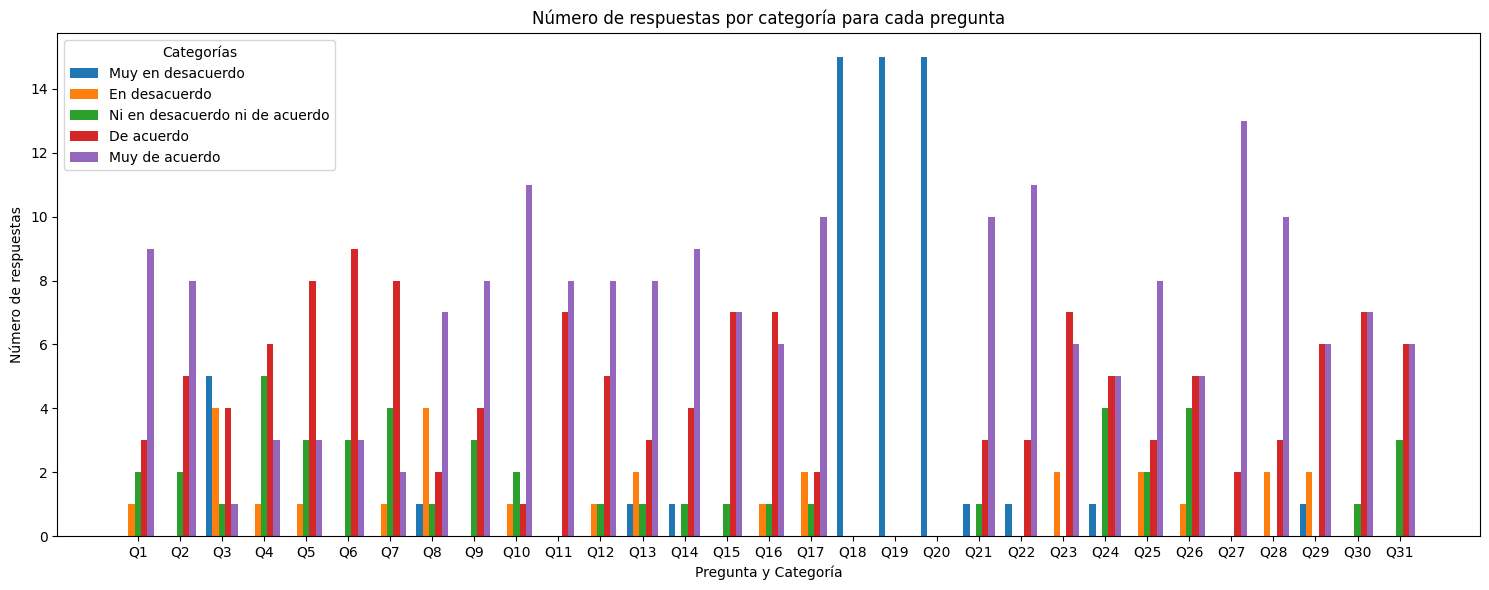
\includegraphics[scale=.5]{imagenes/answers.png}
	\caption{Agregación de respuestas por categoría y por pregunta}
	\label{RespuestasAgregadas}
\end{figure}

Por otra parte, en \cite{meegaplus} se utiliza Item Response Theory (IRT) para asignar un valor $\theta$ para la calidad del juego. Este se calcula a través de un script de R entregado en la \href{http://www.gqs.ufsc.br/quality-evaluation/meega-plus/}{\text{página del Software Quality Group de la Universidad Federal Santa Catarina de Brasil}} \cite{meegaplusQualityEvaluationPage}.

En tal página, se entrega un archivo de parámetros que pondera cada pregunta, además de asignar un valor de dificultad de elección entre cada item. Es decir, indica qué tan difícil es que un usuario se encuentre entre responder, por ejemplo, muy en desacuerdo y de acuerdo, facilitando la distinción entre opiniones.




\section{Resultados de la encuesta libre}

Todavía en curso. Se mostrará otro gráfico como le de la figura \ref{RespuestasAgregadas}.
% TODO: Publicar aquí los resultados de la encuesta libre